\documentclass[border=3pt,tikz]{standalone}
\usepackage{amsmath}
\usetikzlibrary{arrows.meta}
\usetikzlibrary{calc}
\begin{document}
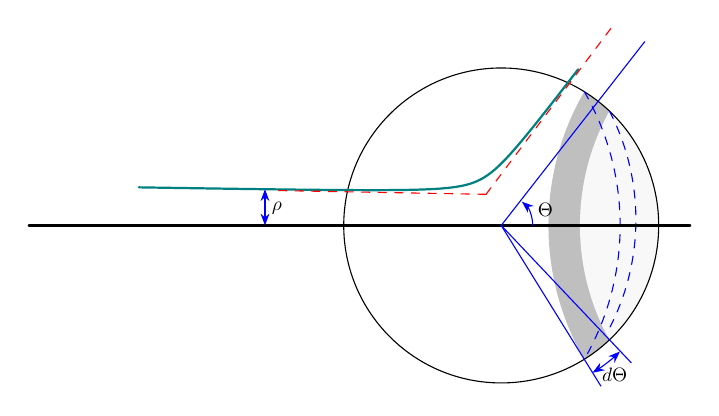
\begin{tikzpicture}[line cap=round, scale = 2]
%\begin{scope}
%  \clip (0,0) circle (1);
%  \fill[gray!20] (-0.625,0) circle (1.5);
%  \fill[gray!0] (-0.945,0) circle (1.7);
%\end{scope}

\begin{scope}
  \clip (0,0) circle (1cm);
  \fill[gray!50] (2.0,0) circle (1.7);
  \fill[gray!0, opacity = 0.9] (2.0,0) circle (1.5);
\end{scope}

\def\e{2.2};
\def\a{0.1};
\def\s{sqrt(\e*\e-1)};

\draw (0,0) circle (1cm);

\draw [blue, dashed] (0.5275,0.8500) arc (30:-30:1.7);
\draw [blue, dashed] (0.6875,0.726) arc (27.35:-27.35:1.5);

\draw [thick] (-3, 0) -- (1.2, 0);

\draw [blue] (0, 0) -- ($1.5 *(0.6075, 0.778)$);
\draw [blue, -{Stealth[length=1.5mm]}] (0.2, 0) arc (0:49.1:0.2);
\node [scale = 0.7] at (0.28, 0.1) {$\Theta$}; 
\draw [blue] (0, 0) -- ($1.2*(0.5275, -0.8500)$);
\draw [blue] (0, 0) -- ($1.2*(0.6875, -0.726)$);
\draw [blue, {Stealth[length=1.5mm]}-{Stealth[length=1.5mm]}] (0.580, -0.935) arc (-58:-46.5:1.1);
\node [scale = 0.7] at (0.72, -0.95) {$d\Theta$};

\begin{scope}[rotate=116]
\coordinate (A) at (-1, 0);
\draw[teal, thick] plot[variable=\t,domain=-2.2:3, samples=100, smooth,thick] ({\a * (cosh(\t) + \e)}, {\a * sqrt(\e*\e-1)*sinh(\t)});

\draw[red, dashed] (\a * \e, 0) -- ({\a * \e + 0.6},  { 0.6 * sqrt(\e*\e-1) });
\draw[red, dashed] (\a * \e, 0) -- ({\a * \e + 0.6},  { -0.6 * sqrt(\e*\e-1) });
\end{scope}

\draw [blue, {Stealth[length=1.5mm]}-{Stealth[length=1.5mm]}] (-1.5, 0) -- (-1.5, 0.23);
\node [right, scale=0.7] at (-1.5, 0.11) {$\rho$};
\end{tikzpicture}
\end{document}